\chapter{Cinétique chimique~: lois de vitesse}\label{ch:b1:rate-laws}

Le lait se conserve une semaine au réfrigérateur et une journée sur une
table en été. La boîte d'un médicament porte la mention «~à conserver à
une température inférieure à \qty{25}{\celsius}~» et une date de
péremption fixée deux ou trois ans plus tard, que le fabricant n'a pas eu
le temps d'observer directement. Les constantes d'équilibre disent où
s'arrête une réaction~; elles ne disent rien du temps qu'il faut pour y
parvenir. C'est le domaine de la cinétique chimique. Ce chapitre définit
la vitesse d'une réaction, les \omterm{def:b1:rate-laws:order}{lois de vitesse} qui l'expriment en
fonction des concentrations, les formes intégrées qui prévoient les
concentrations à tout instant, les méthodes expérimentales qui
déterminent une \omterm{def:b1:rate-laws:order}{loi de vitesse}, et la \omterm{thm:b1:rate-laws:arrhenius}{loi d'Arrhenius} qui décrit l'effet
de la température --- l'outil grâce auquel on prévoit en quelques
semaines d'expériences la durée de conservation d'un médicament.

\begin{recall}
Le livre 1 (année 12) a introduit les vitesses d'apparition et de
disparition d'une espèce, les facteurs cinétiques (concentration,
température, catalyseur) et le \omterm{def:b1:rate-laws:half-life}{temps de demi-réaction} d'une réaction
d'ordre 1. L'\omterm{def:b1:extent-q-and-k:extent}{avancement} $\xi$ d'une réaction a été défini à la
\cref{def:b1:extent-q-and-k:extent}.
\end{recall}

\begin{omfigure}
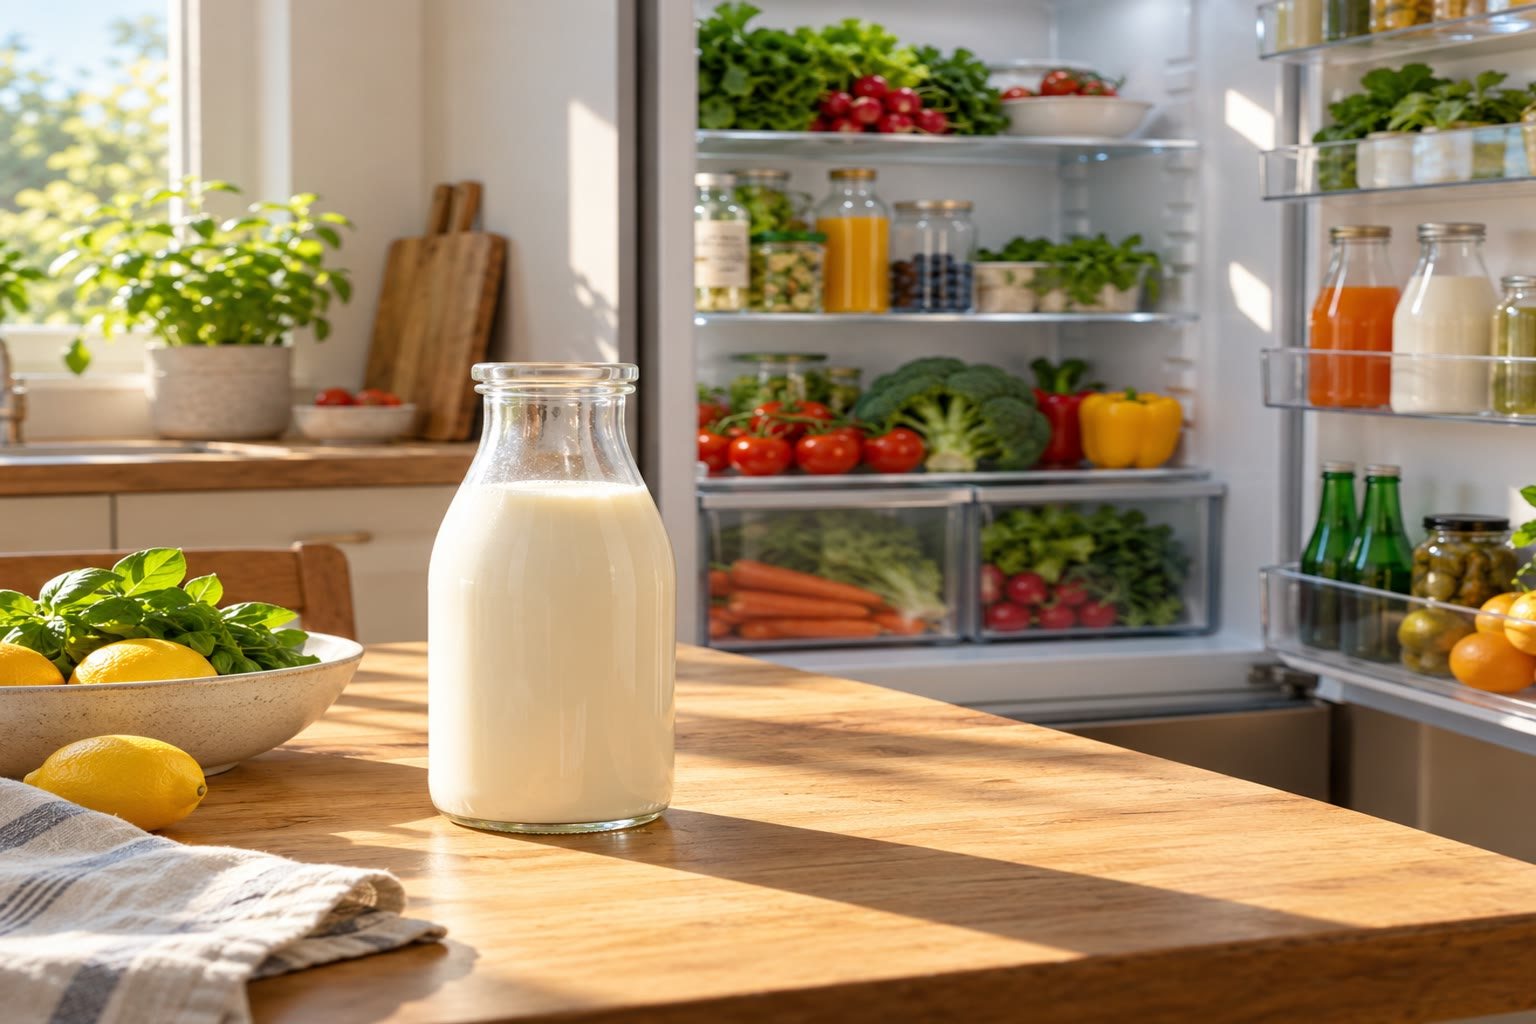
\includegraphics[width=0.55\linewidth]{images/book2/ai/b1-08-milk-kitchen.jpg}

{\small Une bouteille de lait laissée au soleil à côté d'un réfrigérateur
ouvert. Les réactions qui l'altèrent sont plusieurs fois plus rapides à
la température d'un été qu'au froid.}
\end{omfigure}

\section{La vitesse d'une réaction}

\begin{definition}[Vitesse de réaction, vitesses de formation et de disparition]\label{def:b1:rate-laws:rate}
Pour une réaction $0 = \sum_i \nu_i\mathrm{A}_i$ qui se déroule dans un
réacteur fermé de volume $V$ constant, la \emph{vitesse de réaction}\index{vitesse de reaction@vitesse de réaction}
vaut
\[
  v = \frac{1}{V}\frac{\dd\xi}{\dd t} = \frac{1}{\nu_i}\frac{\dd[\mathrm{A}_i]}{\dd t}
  \quad\text{(quel que soit } i\text{)},
\]
en \unit{mol.L^{-1}.s^{-1}}. La \emph{vitesse de formation}\index{vitesse de formation}
d'un produit est $\dd[\mathrm{A}_i]/\dd t$~; la \emph{vitesse de
disparition}\index{vitesse de disparition} d'un réactif est
$-\dd[\mathrm{A}_i]/\dd t$.
\end{definition}

\begin{proposition}[Une seule vitesse pour toutes les espèces]\label{prop:b1:rate-laws:rate-relations}
La \omterm{def:b1:rate-laws:rate}{vitesse de réaction} ne dépend pas de l'espèce choisie pour la suivre~:
pour $a\,\mathrm{A} + b\,\mathrm{B} \longrightarrow c\,\mathrm{C} + d\,\mathrm{D}$,
\[
  v = -\frac1a\frac{\dd[\ce{A}]}{\dd t} = -\frac1b\frac{\dd[\ce{B}]}{\dd t}
  = \frac1c\frac{\dd[\ce{C}]}{\dd t} = \frac1d\frac{\dd[\ce{D}]}{\dd t} .
\]
\end{proposition}

\begin{proof}
$[\mathrm{A}_i] = (n_{i,0} + \nu_i\xi)/V$ avec $V$ constant, donc
$\dd[\mathrm{A}_i]/\dd t = (\nu_i/V)\,\dd\xi/\dd t = \nu_i v$.
\end{proof}

\begin{example}[Décomposition du pentaoxyde de diazote]\label{ex:b1:rate-laws:n2o5}
Pour \ce{2N2O5 -> 4NO2 + O2}~: $v = -\frac12\frac{\dd[\ce{N2O5}]}{\dd t} =
\frac14\frac{\dd[\ce{NO2}]}{\dd t} = \frac{\dd[\ce{O2}]}{\dd t}$. Le
dioxyde d'azote apparaît quatre fois plus vite que le dioxygène, et le
pentaoxyde de diazote disparaît deux fois plus vite que le dioxygène
n'apparaît.
\end{example}

\section{Lois de vitesse et ordres}

\begin{definition}[Loi de vitesse, ordres, constante de vitesse]\label{def:b1:rate-laws:order}
Une \emph{loi de vitesse}\index{loi de vitesse} exprime la vitesse en fonction des
concentrations. Une réaction \emph{admet un ordre} lorsque sa loi de
vitesse est de la forme
\[
  v = k\,[\mathrm{A}]^{p}\,[\mathrm{B}]^{q} \cdots ;
\]
les exposants $p$, $q$, \dots\ sont les \emph{ordres partiels}\index{ordre partiel}
par rapport à A, B, \dots, leur somme est l'\emph{ordre
global}\index{ordre global}, et $k$ est la \emph{constante de vitesse}\index{constante de vitesse},
qui ne dépend que de la température. Les ordres se déterminent par
l'expérience~; ils ne sont pas nécessairement égaux aux coefficients
stœchiométriques, et ils peuvent être fractionnaires ou nuls.
\end{definition}

\begin{remark}[Unités de $k$]\label{rem:b1:rate-laws:units}
Comme $v$ s'exprime en \unit{mol.L^{-1}.s^{-1}}, $k$ s'exprime en
\unit{mol.L^{-1}.s^{-1}} pour l'ordre 0, en \unit{s^{-1}} pour l'ordre 1,
en \unit{L.mol^{-1}.s^{-1}} pour l'ordre 2, et en général en
$(\unit{mol/L})^{1-n}\,\unit{s^{-1}}$ pour l'\omterm{def:b1:rate-laws:order}{ordre global} $n$. L'unité
de $k$ indique l'\omterm{def:b1:rate-laws:order}{ordre global}.
\end{remark}

\begin{remark}[Réactions sans ordre]\label{rem:b1:rate-laws:no-order}
Toutes les réactions n'admettent pas d'ordre. La vitesse de certaines
réactions est une fraction dont le dénominateur contient des
concentrations, ou dépend de la concentration d'un produit. De telles
\omterm{def:b1:rate-laws:order}{lois de vitesse} s'expliquent par le mécanisme de la réaction
(\cref{ch:b1:elementary-steps}). Une réaction peut aussi n'admettre un
ordre qu'au début~: on parle d'ordre initial.
\end{remark}

\section{Lois de vitesse intégrées et temps de demi-réaction}

\begin{definition}[Temps de demi-réaction]\label{def:b1:rate-laws:half-life}
Le \emph{temps de demi-réaction}\index{temps de demi-reaction@temps de demi-réaction} $t_{1/2}$ d'un réactif est
la durée au bout de laquelle la moitié de sa quantité initiale a été
consommée.
\end{definition}

\begin{theorem}[Lois de vitesse intégrées]\label{thm:b1:rate-laws:integrated}
Pour une réaction $a\mathrm{A} \rightarrow \text{produits}$ de vitesse $v = -\frac1a\frac{\dd[\ce{A}]}
{\dd t} = k[\ce{A}]^n$, avec $[\ce{A}](0) = a_0$~:
\begin{center}
\begin{tabular}{llll}
\hline
ordre & loi intégrée & représentation linéaire & \omterm{def:b1:rate-laws:half-life}{temps de demi-réaction} \\
\hline
0 & $[\ce{A}] = a_0 - akt$ & $[\ce{A}]$ en fonction de $t$ & $a_0/(2ak)$ \\
1 & $[\ce{A}] = a_0\,\eu^{-akt}$ & $\ln[\ce{A}]$ en fonction de $t$ & $\ln2/(ak)$ \\
2 & $\dfrac{1}{[\ce{A}]} = \dfrac{1}{a_0} + akt$ & $1/[\ce{A}]$ en fonction de $t$ & $1/(ak\,a_0)$ \\
\hline
\end{tabular}
\end{center}
\end{theorem}

\begin{proof}
Posons $c = [\ce{A}]$, de sorte que $\dd c/\dd t = -akc^n$.
\emph{Ordre 0}~: $\dd c/\dd t = -ak$, d'où $c = a_0 - akt$ (valable
jusqu'à $c = 0$). \emph{Ordre 1}~: $\dd c/\dd t = -akc$ est une
équation différentielle linéaire du premier ordre, de solution
$c = a_0\eu^{-akt}$.
\emph{Ordre 2}~: $\dd c/c^2 = -ak\,\dd t$~; en intégrant de 0 à $t$,
$-1/c + 1/a_0 = -akt$, donc $1/c = 1/a_0 + akt$. \omterm{def:b1:rate-laws:half-life}{Temps de
demi-réaction}~: poser $c =
a_0/2$ dans chaque loi et résoudre en $t$.
\end{proof}

\begin{proposition}[Le test du temps de demi-réaction]\label{prop:b1:rate-laws:half-life-test}
Le \omterm{def:b1:rate-laws:half-life}{temps de demi-réaction} est indépendant de la concentration initiale
si et seulement si la réaction est d'ordre 1. Il est proportionnel à
$a_0$ pour l'ordre 0 et à $1/a_0$ pour l'ordre 2. Une réaction d'ordre 1
perd la moitié de ce qui reste à chaque nouveau \omterm{def:b1:rate-laws:half-life}{temps de demi-réaction}~:
au bout de $m$ \omterm{def:b1:rate-laws:half-life}{temps de demi-réaction}, il reste une fraction $2^{-m}$.
\end{proposition}

\begin{proof}
Pour un ordre $n \ne 1$, la séparation des variables donne $t_{1/2} = \dfrac{2^{n-1} -
1}{(n-1)\,ak\,a_0^{n-1}}$, qui dépend de $a_0$ sauf si $n = 1$~; pour
$n = 1$, $t_{1/2} = \ln2/(ak)$. Pour l'ordre 1, $c(t + t_{1/2}) = c(t)/2$
à tout instant $t$, puisque $\eu^{-ak(t + t_{1/2})} = \eu^{-akt}/2$.
\end{proof}

\begin{omfigure}
\begin{tikzpicture}
\begin{axis}[name=p0,
  width=0.36\linewidth, height=4.6cm,
  xmin=0, xmax=60, ymin=0, ymax=1.05,
  axis x line=bottom, axis y line=left,
  xlabel={$t$ (min)}, title={ordre 0~: $[\ce{A}]$},
  title style={font=\small}, xtick={0,20,40,60},
  tick label style={font=\scriptsize}, label style={font=\small}]
\addplot[omDef, thick] table[x=t, y=A0] {figdata/out/bachelor-1-integrated-rate-laws.dat};
\end{axis}
\begin{axis}[at={(p0.east)}, anchor=west, xshift=0.9cm, name=p1,
  width=0.36\linewidth, height=4.6cm,
  xmin=0, xmax=60, ymin=-3.2, ymax=0.2,
  axis x line=bottom, axis y line=left,
  xlabel={$t$ (min)}, title={ordre 1~: $\ln[\ce{A}]$},
  title style={font=\small}, xtick={0,20,40,60},
  tick label style={font=\scriptsize}, label style={font=\small}]
\addplot[omProp, thick] table[x=t, y=lnA1] {figdata/out/bachelor-1-integrated-rate-laws.dat};
\end{axis}
\begin{axis}[at={(p1.east)}, anchor=west, xshift=0.9cm,
  width=0.36\linewidth, height=4.6cm,
  xmin=0, xmax=60, ymin=0, ymax=4.2,
  axis x line=bottom, axis y line=left,
  xlabel={$t$ (min)}, title={ordre 2~: $1/[\ce{A}]$},
  title style={font=\small}, xtick={0,20,40,60},
  tick label style={font=\scriptsize}, label style={font=\small}]
\addplot[omThm, thick] table[x=t, y=invA2] {figdata/out/bachelor-1-integrated-rate-laws.dat};
\end{axis}
\end{tikzpicture}

\begin{tikzpicture}
\begin{axis}[
  width=0.62\linewidth, height=5.0cm,
  xmin=0, xmax=60, ymin=0, ymax=1.05,
  axis x line=bottom, axis y line=left,
  xlabel={$t$ (min)}, ylabel={$[\ce{A}]$ (mol/L)}, xtick={0,10,20,30,40,50,60},
  tick label style={font=\small}, label style={font=\small},
  legend style={font=\small, draw=none, at={(0.98,0.98)}, anchor=north east}]
\addplot[omDef, thick] table[x=t, y=A0] {figdata/out/bachelor-1-integrated-rate-laws.dat};
\addplot[omProp, thick] table[x=t, y=A1] {figdata/out/bachelor-1-integrated-rate-laws.dat};
\addplot[omThm, thick] table[x=t, y=A2] {figdata/out/bachelor-1-integrated-rate-laws.dat};
\legend{ordre 0, ordre 1, ordre 2}
\draw[dotted] (axis cs:0,0.5) -- (axis cs:20,0.5);
\end{axis}
\end{tikzpicture}

{\small Trois réactions de même concentration initiale
(\qty{1.00}{mol/L}) et de même \omterm{def:b1:rate-laws:initial-rate}{vitesse initiale}
(\qty{0.050}{mol.L^{-1}.min^{-1}}). En haut~: chaque loi intégrée devient
une droite dans ses propres coordonnées. En bas~: les concentrations~;
les \omterm{def:b1:rate-laws:half-life}{temps de demi-réaction} valent 10, 13.9 et 20 minutes.}
\end{omfigure}

\section{Déterminer une loi de vitesse}

\begin{method}[La méthode intégrale]\label{met:b1:rate-laws:integral}
Pour tester un ordre à partir de mesures de $[\ce{A}](t)$~: tracer
$[\ce{A}]$, $\ln[\ce{A}]$ et $1/[\ce{A}]$ en fonction de $t$~; la
représentation qui est une droite donne l'ordre, et sa pente donne $k$
(pente $-ak$, $-ak$ ou $+ak$ respectivement).
\end{method}

\begin{method}[La méthode des temps de demi-réaction]\label{met:b1:rate-laws:half-life}
Mesurer le \omterm{def:b1:rate-laws:half-life}{temps de demi-réaction} pour plusieurs concentrations
initiales~: constant, ordre 1~; proportionnel à $a_0$, ordre 0~;
proportionnel à $1/a_0$, ordre 2. Dans une seule expérience, comparer les
durées pour passer de $a_0$ à $a_0/2$ et de $a_0/2$ à $a_0/4$~: des
durées égales signifient l'ordre 1.
\end{method}

\begin{definition}[Vitesse initiale]\label{def:b1:rate-laws:initial-rate}
La \emph{vitesse initiale}\index{vitesse initiale} $v_0$ est la vitesse à $t = 0$,
lue comme la pente de la tangente à l'origine de la courbe $[\ce{A}](t)$,
divisée par le coefficient stœchiométrique. À cet instant, les
concentrations sont les concentrations initiales, connues, et aucun
produit n'interfère.
\end{definition}

\begin{method}[La méthode des vitesses initiales]\label{met:b1:rate-laws:initial-rates}
Pour $v_0 = k[\ce{A}]_0^p[\ce{B}]_0^q$~: réaliser des expériences où
l'on ne fait varier que $[\ce{A}]_0$~; alors
$\ln v_0 = \ln(k[\ce{B}]_0^q) + p\ln[\ce{A}]_0$,
et la pente de $\ln v_0$ en fonction de $\ln[\ce{A}]_0$ vaut $p$. En
pratique, doubler $[\ce{A}]_0$ multiplie $v_0$ par $2^p$. Faire de même
pour B.
\end{method}

\begin{definition}[Méthode d'isolement, ordre apparent]\label{def:b1:rate-laws:apparent-order}
Dans la \emph{méthode d'isolement}\index{methode d'isolement@méthode d'isolement}, tous les réactifs sauf un
sont introduits en large excès (dix fois ou plus). Leurs concentrations
restent pratiquement constantes, et
$v = k[\ce{A}]^p[\ce{B}]^q \approx k'[\ce{A}]^p$
avec $k' = k[\ce{B}]_0^q$~: la réaction se comporte comme si elle était
d'\emph{ordre apparent}\index{ordre apparent} $p$, avec la \omterm{def:b1:rate-laws:order}{constante de vitesse}
apparente $k'$. On parle aussi de dégénérescence de l'ordre.
\end{definition}

\begin{omfigure}
\begin{tikzpicture}
\begin{axis}[
  width=0.55\linewidth, height=4.8cm,
  xmin=0, xmax=40, ymin=0, ymax=1.05,
  axis x line=bottom, axis y line=left,
  xlabel={$t$ (min)}, ylabel={$[\ce{A}]$ (mol/L)},
  xtick={0,10,20,30,40},
  tick label style={font=\small}, label style={font=\small}, clip mode=individual]
\addplot[omProp, thick] table[x=t, y=A1] {figdata/out/bachelor-1-integrated-rate-laws.dat};
\draw[omThm, thick] (axis cs:0,1) -- (axis cs:20,0);
\node[omThm, anchor=west, font=\small] at (axis cs:2,0.12) {tangente en $t = 0$};
\end{axis}
\end{tikzpicture}

{\small Lecture d'une \omterm{def:b1:rate-laws:initial-rate}{vitesse initiale}~: la tangente à l'origine (en
rouge) d'une courbe d'ordre 1 coupe l'axe des temps en
$t_0 = \qty{20}{min}$, donc $v_0 =
\qty{1.00}{mol/L}/\qty{20}{min} = \qty{0.050}{mol.L^{-1}.min^{-1}}$.}
\end{omfigure}

\begin{inthelab}[Suivre une réaction au cours du temps]
Une \omterm{def:b1:rate-laws:order}{loi de vitesse} se construit à partir de concentrations mesurées
pendant que la réaction se déroule. Lorsqu'un réactif ou un produit est
coloré, un spectrophotomètre enregistre l'absorbance, proportionnelle à
sa concentration (Beer--Lambert, \cref{ch:b1:structure-spectroscopy})~;
lorsque des ions apparaissent ou disparaissent, un conductimètre suit la
conductivité~; lorsqu'un gaz se forme dans un récipient fermé, un
manomètre suit la pression. Sinon, on prélève des échantillons à des
instants connus, on arrête la réaction (trempe) par refroidissement ou
dilution, et l'on titre chaque échantillon. La température du récipient
est maintenue constante par un bain thermostaté, car $k$ en dépend
fortement.
\end{inthelab}

\section{Température~: la loi d'Arrhenius}

\begin{definition}[Énergie d'activation]\label{def:b1:rate-laws:activation-energy}
L'\emph{énergie d'activation}\index{energie d'activation@énergie d'activation} $E_a$ d'une réaction de
\omterm{def:b1:rate-laws:order}{constante de vitesse} $k(T)$ est définie par
\[
  \frac{\dd \ln k}{\dd T} = \frac{E_a}{RT^2} ,
\]
en \unit{J/mol}. Lorsque $E_a$ est indépendante de $T$, l'intégration
donne $k = A\,\eu^{-E_a/RT}$, où la constante $A$, de même unité que
$k$, est le \emph{facteur préexponentiel}\index{facteur preexponentiel@facteur préexponentiel}.
\end{definition}

\begin{theorem}[Loi d'Arrhenius]\label{thm:b1:rate-laws:arrhenius}
Pour la plupart des réactions, sur un domaine de température modéré, la
\omterm{def:b1:rate-laws:order}{constante de vitesse} suit la \emph{loi d'Arrhenius}\index{loi d'Arrhenius}
\[
  k(T) = A\,\eu^{-E_a/RT} ,
\]
avec $A$ et $E_a > 0$ indépendants de $T$~: $\ln k$ est une fonction
affine de $1/T$, de pente $-E_a/R$.
\end{theorem}
\admitted

\begin{remark}[Le sens de $E_a$]\label{rem:b1:rate-laws:meaning}
La loi est empirique. Son interprétation --- seuls les chocs entre
molécules qui apportent au moins une énergie de l'ordre de $E_a$ mènent
à la réaction, et la fraction de tels chocs varie comme $\eu^{-E_a/RT}$
--- est esquissée avec les profils énergétiques du chapitre suivant et
rendue quantitative par les théories de la \omterm{def:b1:rate-laws:rate}{vitesse des réactions} dans le
volume de troisième année.
\end{remark}

\begin{method}[Déterminer $E_a$]\label{met:b1:rate-laws:arrhenius-plot}
À partir de \omterm{def:b1:rate-laws:order}{constantes de vitesse} à plusieurs températures, tracer
$\ln k$ en fonction de $1/T$ (en kelvins)~: la pente vaut $-E_a/R$,
l'ordonnée à l'origine $\ln A$. Avec deux températures seulement,
\[
  E_a = \frac{R\,\ln(k_2/k_1)}{1/T_1 - 1/T_2} .
\]
\end{method}

\begin{example}[Une règle empirique]\label{ex:b1:rate-laws:doubling}
Pour $E_a = \qty{53}{kJ/mol}$, passer de 25 à \qty{35}{\celsius}
multiplie $k$ par $\exp\!\big(\frac{53000}{8.314}(\frac{1}{298.15} -
\frac{1}{308.15})\big) = 2.0$. La règle bien connue «~dix degrés de
plus, deux fois plus vite~» vaut près de la température ambiante pour
les réactions dont l'\omterm{def:b1:rate-laws:activation-energy}{énergie d'activation} avoisine \qty{50}{kJ/mol}~;
pour une $E_a$ plus grande, le facteur est plus grand.
\end{example}

\begin{omfigure}
\begin{tikzpicture}
\begin{axis}[
  width=0.6\linewidth, height=5.4cm,
  xmin=2.95, xmax=3.45, ymin=-9.0, ymax=-4.2, clip mode=individual,
  axis x line=bottom, axis y line=left,
  xlabel={$1000/T$ (\unit{K^{-1}})}, ylabel={$\ln k$ ($k$ en \unit{d^{-1}})},
  xtick={3.0,3.1,3.2,3.3,3.4}, ytick={-9,-8,-7,-6,-5},
  tick label style={font=\small}, label style={font=\small}]
\addplot[omDef, thick] table[x=invT_1e3, y=lnk] {figdata/out/bachelor-1-arrhenius-line.dat};
\addplot[only marks, mark=*, mark size=2.2pt, omThm] table[x=invT_1e3, y=lnk] {figdata/out/bachelor-1-arrhenius-points.dat};
\node[font=\small, anchor=south west] at (axis cs:3.002,-4.71) {\qty{60}{\celsius}};
\node[font=\small, anchor=south west] at (axis cs:3.095,-5.66) {\qty{50}{\celsius}};
\node[font=\small, anchor=south west] at (axis cs:3.193,-6.67) {\qty{40}{\celsius}};
\draw[dashed, black!50] (axis cs:3.354,-9.0) -- (axis cs:3.354,-8.31);
\addplot[only marks, mark=o, mark size=2.4pt, omDef] coordinates {(3.354,-8.310)};
\node[font=\small, anchor=east] at (axis cs:3.33,-8.40) {\qty{25}{\celsius}, extrapolé};
\end{axis}
\end{tikzpicture}

{\small Droite d'Arrhenius de la dégradation d'un médicament (problème
du week-end)~: trois \omterm{def:b1:rate-laws:order}{constantes de vitesse} mesurées (en rouge) sont
alignées sur une droite de pente $-E_a/R$~; extrapolée à
\qty{25}{\celsius}, elle donne la durée de conservation à température
ambiante.}
\end{omfigure}

\begin{history}[Arrhenius, 1889]
Le chimiste suédois Svante Arrhenius, qui étudiait en 1889 l'inversion du
saccharose par les acides, proposa que seule une petite fraction des
molécules, celles qui se trouvent dans un état «~activé~», réagissent,
et que cette fraction croît avec la température comme $\eu^{-E/RT}$.
L'idée, d'abord contestée, devint le fondement de la cinétique
chimique. Arrhenius reçut le prix Nobel de chimie en 1903, pour sa
théorie de la dissociation électrolytique.
\end{history}

\begin{omfigure}
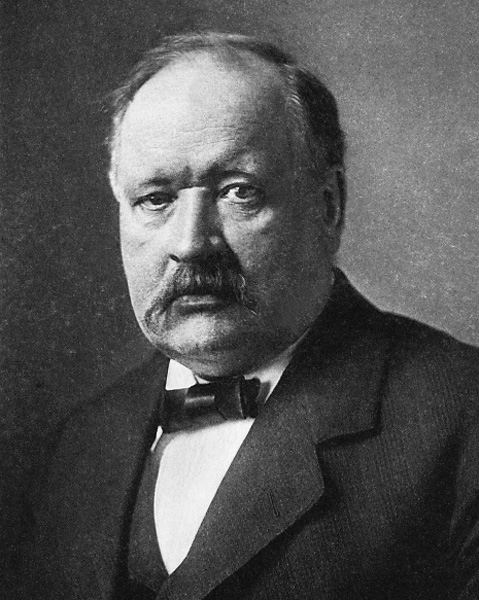
\includegraphics[width=0.22\linewidth]{images/book2/arrhenius.jpg}

{\small Svante Arrhenius (1859--1927), en 1909.}
\end{omfigure}

\section{Exercices}

\begin{exercise}[$\star$]\label{exo:b1:rate-laws:1}
Pour \ce{2N2O5 -> 4NO2 + O2} à volume constant, le dioxyde d'azote
apparaît à $\qty{2.0e-4}{mol.L^{-1}.s^{-1}}$. Donner la \omterm{def:b1:rate-laws:rate}{vitesse de
réaction}, la \omterm{def:b1:rate-laws:rate}{vitesse de formation} du dioxygène et la \omterm{def:b1:rate-laws:rate}{vitesse de
disparition} de \ce{N2O5}.
\end{exercise}

\begin{exercise}[$\star$]\label{exo:b1:rate-laws:2}
Donner l'unité de la \omterm{def:b1:rate-laws:order}{constante de vitesse} pour les ordres globaux 0, 1, 2
et 3, les concentrations étant en \unit{mol/L} et les temps en secondes.
\end{exercise}

\begin{exercise}[$\star$]\label{exo:b1:rate-laws:3}
Une réaction d'ordre 1 $\mathrm{A} \longrightarrow \mathrm{B}$ a pour
constante $k = \qty{3.0e-3}{s^{-1}}$. Calculer son \omterm{def:b1:rate-laws:half-life}{temps de
demi-réaction} et la fraction de \ce{A} restant au bout de \qty{10}{min}.
\end{exercise}

\begin{exercise}[$\star$]\label{exo:b1:rate-laws:4}
Quand la concentration initiale d'un réactif est divisée par deux, son
\omterm{def:b1:rate-laws:half-life}{temps de demi-réaction} double. Quel est l'ordre~? Et si le \omterm{def:b1:rate-laws:half-life}{temps de
demi-réaction} est divisé par deux~?
\end{exercise}

\begin{exercise}[$\star\star$]\label{exo:b1:rate-laws:5}
On mesure la concentration d'un réactif \ce{A}
($\mathrm{A} \longrightarrow \mathrm{P}$)~: à $t
= 0$, 10, 20, 30 et \qty{40}{min}, $[\ce{A}] = 0.100$, 0.0741, 0.0549,
0.0407 et \qty{0.0301}{mol/L}. Déterminer l'ordre et la \omterm{def:b1:rate-laws:order}{constante de
vitesse}.
\end{exercise}

\begin{exercise}[$\star\star$]\label{exo:b1:rate-laws:6}
Pour $\mathrm{A} + \mathrm{B} \longrightarrow \mathrm{P}$, $v_0 = \qty{2.0e-6}{mol.L^{-1}.s^{-1}}$ pour $[\ce{A}]_0
= [\ce{B}]_0 = \qty{0.010}{mol/L}$~; \qty{8.0e-6}{} quand $[\ce{A}]_0$
est doublée~; \qty{4.0e-6}{} quand $[\ce{B}]_0$ est doublée. Déterminer
les \omterm{def:b1:rate-laws:order}{ordres partiels}, la \omterm{def:b1:rate-laws:order}{loi de vitesse} et la \omterm{def:b1:rate-laws:order}{constante de vitesse}.
\end{exercise}

\begin{exercise}[$\star\star$]\label{exo:b1:rate-laws:7}
La \omterm{def:b1:rate-laws:order}{loi de vitesse} de $\mathrm{A} + \mathrm{B} \longrightarrow \mathrm{P}$
est $v = k[\ce{A}][\ce{B}]$. Avec
$[\ce{B}]_0 = \qty{0.50}{mol/L}$ et $[\ce{A}]_0 = \qty{5.0e-3}{mol/L}$,
\ce{A} disparaît selon une cinétique d'ordre 1, avec une constante
apparente de \qty{0.012}{s^{-1}}. Expliquer et calculer $k$.
\end{exercise}

\begin{exercise}[$\star\star$]\label{exo:b1:rate-laws:8}
Une \omterm{def:b1:rate-laws:order}{constante de vitesse} vaut \qty{1.0e-3}{s^{-1}} à \qty{300}{K} et
\qty{5.0e-3}{s^{-1}} à \qty{320}{K}. Calculer l'\omterm{def:b1:rate-laws:activation-energy}{énergie d'activation} et
la \omterm{def:b1:rate-laws:order}{constante de vitesse} à \qty{310}{K}.
\end{exercise}

\begin{exercise}[$\star\star$]\label{exo:b1:rate-laws:9}
La réaction $2\,\mathrm{A} \longrightarrow \mathrm{P}$ a pour \omterm{def:b1:rate-laws:order}{loi de
vitesse} $v = -\frac12\frac{\dd[\ce{A}]}
{\dd t} = k[\ce{A}]^2$ avec $k = \qty{0.50}{L.mol^{-1}.s^{-1}}$. À
partir de $[\ce{A}]_0 = \qty{0.020}{mol/L}$, calculer le \omterm{def:b1:rate-laws:half-life}{temps de
demi-réaction} et la concentration au bout de \qty{100}{s}.
\end{exercise}

\begin{exercise}[$\star\star\star$]\label{exo:b1:rate-laws:10}
Pour une réaction d'ordre 1, montrer que la durée nécessaire pour
consommer une fraction $f$ du réactif vaut $t_f = -\ln(1 - f)/(ak)$.
Comparer les durées pour 50\,\%, 75\,\%, 90\,\% et 99.9\,\%, en \omterm{def:b1:rate-laws:half-life}{temps de
demi-réaction}.
\end{exercise}

\begin{exercise}[$\star\star\star$]\label{exo:b1:rate-laws:11}
Un patch cutané libère un médicament à la vitesse constante de
\qty{0.40}{mg/h} tant que son réservoir, initialement de \qty{10}{mg},
n'est pas vide. Écrire la loi donnant la quantité restante, donner son
ordre, son \omterm{def:b1:rate-laws:half-life}{temps de demi-réaction} et la durée au bout de laquelle le
patch est épuisé. Pourquoi une cinétique d'ordre zéro convient-elle à un
patch médicamenteux~?
\end{exercise}

\begin{exercise}[$\star\star\star$]\label{exo:b1:rate-laws:12}
Montrer que la règle «~dix degrés de plus, deux fois plus vite~» entre
\qty{298.15}{K} et \qty{308.15}{K} correspond à $E_a \approx
\qty{53}{kJ/mol}$. Quel facteur la même \omterm{def:b1:rate-laws:activation-energy}{énergie d'activation} donne-t-elle
entre \qty{0}{\celsius} et \qty{10}{\celsius}~?
\end{exercise}

\section{Problème~: la durée de conservation d'un médicament}

\begin{problem}[{Problème du week-end --- un test de stabilité accéléré~:
dégradation d'ordre 1 à 60\,\textdegree C, trois températures, la droite
d'Arrhenius, et la durée de conservation à température ambiante}]
\label{pb:b1:rate-laws:1}
Pour prévoir la durée de conservation $t_{90}$ d'un comprimé (la durée
au bout de laquelle 10\,\% du principe actif s'est dégradé), un
laboratoire stocke des échantillons à haute température et mesure le
pourcentage de principe actif restant. À
\qty{60}{\celsius}~:
\begin{center}
\begin{tabular}{lccccc}
\hline
durée (jours) & 0 & 10 & 20 & 30 & 40 \\
principe actif restant (\%) & 100.0 & 91.4 & 83.5 & 76.3 & 69.8 \\
\hline
\end{tabular}
\end{center}
À 40 et \qty{50}{\celsius}, les \omterm{def:b1:rate-laws:order}{constantes de vitesse} trouvées valent
\qty{1.27e-3}{d^{-1}} et \qty{3.48e-3}{d^{-1}}. Prendre $R =
\qty{8.314}{J/(mol.K)}$ et un mois $= \qty{30.4}{d}$.

\medskip
\noindent\textbf{Partie I --- L'ordre à 60\,\textdegree C.}
\begin{enumerate}
  \item Calculer les pertes sur chaque intervalle de 10 jours. La
        réaction est-elle d'ordre 0~?
  \item Calculer $\ln(\%\text{ restant})$ à chaque instant. Que
        conclure~?
  \item En déduire la \omterm{def:b1:rate-laws:order}{constante de vitesse} $k_{60}$.
  \item Calculer le \omterm{def:b1:rate-laws:half-life}{temps de demi-réaction} à \qty{60}{\celsius}.
  \item Quel pourcentage reste-t-il au bout de 60 jours à
        \qty{60}{\celsius}~?
  \item Calculer $t_{90}$ à \qty{60}{\celsius}.
\end{enumerate}

\medskip
\noindent\textbf{Partie II --- Durée de conservation et ordre.}
\begin{enumerate}[resume]
  \item Montrer que, pour une dégradation d'ordre 1, $t_{90} = \ln(10/9)/k$.
  \item Exprimer $t_{90}$ en fraction du \omterm{def:b1:rate-laws:half-life}{temps de demi-réaction}.
  \item Pourquoi $t_{90}$ ne dépend-il pas du dosage du comprimé~?
  \item Pourquoi les laboratoires mesurent-ils la dégradation à haute
        température plutôt qu'à \qty{25}{\celsius}~?
  \item Si la dégradation était d'ordre 2 par rapport au principe actif,
        un comprimé deux fois plus dosé se conserverait-il plus ou moins
        longtemps~? Expliquer.
\end{enumerate}

\medskip
\noindent\textbf{Partie III --- La droite d'Arrhenius.}
\begin{enumerate}[resume]
  \item Dresser un tableau de $1/T$ et de $\ln k$ pour les trois
        températures.
  \item Calculer la pente de la droite qui passe par les points à 40 et
        à \qty{60}{\celsius}.
  \item En déduire l'\omterm{def:b1:rate-laws:activation-energy}{énergie d'activation}.
  \item Vérifier que le point à \qty{50}{\celsius} est sur la droite.
  \item Calculer le \omterm{def:b1:rate-laws:activation-energy}{facteur préexponentiel} $A$.
  \item De quel facteur la vitesse augmente-t-elle entre 25 et
        \qty{35}{\celsius}~? Comparer à la règle empirique.
\end{enumerate}

\medskip
\noindent\textbf{Partie IV --- La température ambiante.}
\begin{enumerate}[resume]
  \item Extrapoler la \omterm{def:b1:rate-laws:order}{constante de vitesse} à \qty{30}{\celsius}.
  \item Calculer $t_{90}$ à \qty{30}{\celsius}, en mois.
  \item Une boîte est oubliée trois jours dans une voiture à
        \qty{60}{\celsius}. Quelle fraction du principe actif est perdue~?
  \item Expliquer la consigne «~à conserver à une température inférieure
        à \qty{25}{\celsius}~».
  \item Extrapoler la \omterm{def:b1:rate-laws:order}{constante de vitesse} à \qty{25}{\celsius}.
  \item Calculer la durée de conservation $t_{90}$ à \qty{25}{\celsius},
        en jours et en mois.
\end{enumerate}
\end{problem}
